% Facultad de Ingenier\'ia, Universidad de Buenos Aires
% 75.59 Técnicas de Programación Concurrente I

\documentclass[a4paper,12pt,titlepage]{article}
\usepackage[paperwidth=180mm,paperheight=285mm,left=1.5cm,top=4cm,right=1.5cm,bottom=2cm,head=2.0cm,includefoot]{geometry}
\usepackage[spanish]{babel}
%\usepackage[latin1]{inputenc}
\usepackage[utf8]{inputenc}
\usepackage{lscape}
\usepackage{graphicx}
\usepackage{fancyhdr}
\usepackage{rotating}
%\graphicspath{{../}}

\usepackage{listingsutf8}

\title{75.59 Técnicas de Programación Concurrente I, Trabajo Práctico 2}
\author{Torres, Miguel \and Montoya, Diego \and Garay, Ignacio}

\lhead{
\includegraphics[scale=0.06]{./logo_fiuba.pdf}}
\chead{ 75.59 Técnicas de Programación Concurrente I }
\rhead{}

\lfoot{Garay - Montoya - Torres}
\rfoot{\thepage}
\cfoot{$2^{do}$ Cuatrimestre 2013}

\begin{document}

\thispagestyle{empty}
% T\'itulo del documento.
\begin{center}

\includegraphics{./logo-fiuba.png}\\
\vspace{1cm}
\textsc{\LARGE Universidad de Buenos Aires}\\[0.3cm]
\textsc{\LARGE Facultad de Ingenier\'ia}\\[1.2cm]
\textsc{\Large 75.59 - Técnicas de Programación Concurrente I}\\[0.3cm]
\end{center}

\begin{flushright}
{\large
Montoya, Diego -- 91939\\
Torres, Miguel -- 91396\\
Garay, Ignacio -- 92265\\
\vspace{2cm}
$2^{do}$ cuatrimestre de 2013}
\end{flushright}

\pagestyle{fancy}
\setcounter{page}{1}
\newpage

\tableofcontents
\newpage

\footnotesize
\section{Análisis}
En el análisis del trabajo se identificaron las siguientes identidades del dominio:\\
\begin{itemize}
\item Cliente
\item Servidor
\item Receptor de Clientes
\item Resolvedor de Paquetes\\
\end{itemize} 

El Servidor es la clase que inicia todos los recursos necesarios para una tener una conversación, creando además
al Receptor de Clientes y al Resolvedor de Paquetes. El Servidor además es el encargado de de gestionar las 
conversaciones, permitiendo agregar nuevas y administrando las ya existentes.

Cuando un Cliente es iniciado, es el Receptor de Clientes el encargado de iniciar la sesión el mismo con el Servidor, 
dejando todo listo para que el Cliente pueda crear una nueva conversación o unirse a una existente.

Una vez que algunos clientes forman parte de la misma conversación, los mensajes entre ellos enviados son capturados
por el Resolvedor de Paquetes, el cual se encarga de distribuir dichos mensajes a las conversaciones correspondientes.

Puede verse entonces que el Cliente actúa como productor de mensajes, los cuales son consumidos por el Resolvedor
de paquetes, de manera tal que cada uno de ellos llegue a los otros clientes que forman parte de la conversación.

\subsection{Casos de Uso}
Se identificaron además los siguientes casos de uso, desde el punto de vista del usuario:\\
\begin{figure}[h!]
\centering
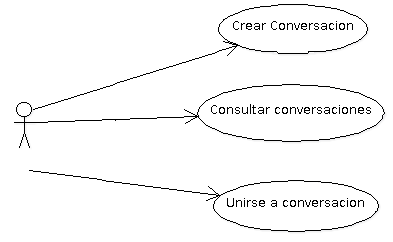
\includegraphics[width=0.6\textwidth]{CasosDeUso.png}
\caption{Diagrama de casos de uso del Cliente}
\label{fig:casos_uso}
\end{figure}

\begin{itemize}
\item \textbf{Crear conversación}\\ 
  Es el caso de uso en el cual un Cliente conectado al Servidor decide iniciar una nueva conversación, en la cual inicialmente
  será el único miembro, hasta que otro Cliente decida unirse para conversar
\item \textbf{Consultar conversaciones}\\
  Es el caso de uso en el cual el Cliente conectado al Servidor decide realizar una consulta sobre las conversaciones
  existentes actualmente en el Servidor
\item \textbf{Unirse a conversación}\\
  Es el caso de uso en el cual un Cliente luego de consultar las conversaciones existentes en el Servidor decide además
  unirse a una de ellas\\
\end{itemize} 


\newpage
\section{Diseño}

Para la resolución de la concurrencia en la aplicacion se implementaron varias herramientas como Fifo, Pipe, Lock , 
Memoria Compartida, Señales y Sockets.

Se creó un proceso encargado de la generacion de los recursos y administración de las conversaciones, llamado 
appServidor, el cual es el punto de inicio de la aplicación\\

También existe el proceso llamado appCliente, el cual es creado cuando un usuario inicia un Cliente y le permite interactuar con
el Servidor para unirse a una conversación o iniciar una nueva\\

Dentro del proceso appServidor se crean 2 nuevos procesos llamados Resolvedor y Recibidor que se encargar de resolver todas la solicitudes 
y recibir nuevos clientes respectivamente.
El funcionamiento del servidor es el siguiente, cuando un cliente intenta conectarse, éste le envia un paquete de inicio de sesión (a traves 
de una conexion UDP), este paquete es captado por el proceso Recibidor, quien crea un nuevo proceso Receptor para ese cliente, luego 
se retransmitirá el paquete y algunos datos más de conexión al proceso Resolvedor y al nuevo Receptor (utilizando un area de memoria compartida). 
Luego el recibidor espera una confirmacion (mediante un semáforo) del proceso Receptor para poder seguir escuchando nuevos usuarios.\\

La tarea que lleva a cabo el proceso resolvedor es almacenar todos los usuarios en linea, todas las conversaciones abiertas y de reenviar 
todos los mensajes que se envien entre si. Para ello cuando arriba un paquete a la Cola de Paquetes (un area de memoria compartida para colocar 
los paquetes de los usuarios que iniciaron sesión) éste lo retira de allí, verifica qué tipo de paquete es, resuelve la petición correspondiente y 
le envía la respuesta al usuario o a todos los integrantes dentro de una conversación si se tratase de un mensaje. Este procedimiento se repite 
hasta que el proceso padre le envie una señal de finalización.\\

Cuando llega una solicitud de inicio de sesión al Resolvedor, éste es informado de la situación mediante una señal que es enviada por el proceso 
Recibidor. La tarea que se lleva a cabo es la siguiente, se lee la información de usuario (paquete y datos de conexion) que fueron colocadas por 
el Recibidor (en un área de memoria compartida). Cuando obtiene el paquete lo procesa (crea el nuevo usuario si no existe) y si no hubo problemas 
se le envía una señal de confirmación al proceso Receptor para que prosiga con su correcta ejecución. En cambio, si otro usuario había iniciado 
sesión con el mismo nombre anteriormente, se emite un error y se le indica al Receptor que finalice, informando sobre este error al usuario. Luego 
de realizar todo esto el proceso Resolvedor finaliza el tratamiento de la señal y continua con su normal ejecución.\\

Los paquetes utilizados en toda la aplicación se diseñaron para resolver varios problemas (como iniciar y finalizar sesión, crear y unirse a una 
conversación, mensajes, etc) y así resolverlos todos contenidos en una misma estructura.
Se pensaron para que sean de tamaño fijo, de 512 bytes concretamente, conformando la siguiente estructura:

\begin{itemize}
\item Cabecera: 2 bytes en formato Big Endian para el tamaño del paquete, 1 byte para el tipo de paquete y 1 ultimo byte para la cantidad de atributos.
\item Datos: 508 bytes disponibles para datos (o tambien llamados atributos).
\end{itemize}\\

Segun el tipo de paquete que sea se resuelve una solicitud diferente. Los diferentes tipos de paquetes son los siguientes:
\begin{itemize}
\item INICIO\_SESION: indica que un usuario intenta inciar sesion.
\item FIN\_SESION: indica que un usuario desea finalizar su sesion.
\item MENSAJE: contiene el mensaje que envio un usuario, en la conversacion donde se encuentra.
\item CREAR\_CONVERSACION: indica que un usuario quiere crear una converasacion.
\item UNIRSE\_CONVERSACION indica que un usuario desea unirse a una conversacion ya creada.
\item CONVERSACIONES: indica una solicitud para que ver las conversaciones disponibles.
\item OK: indica una confirmación sobre algún evento por parte del servidor (inicio y fin de sesion, etc).
\item ERROR: indica un error ocurrido cuando se proceso una solitud de un usuario.
\item DESCONOCIDO: identifica al paquete como desconocido y no se lo puede procesar.

\end{itemize}\\


Se implemento el mismo sistema de log que en primer proyecto, el cual divide los sucesos en diferentes categorías, las cuales son:
\begin{itemize}
\item Info: informacion corriente de los pasos de la ejecucion.
\item Debug: informacion de debug.
\item Fatal: indica una excepcion lanzada.
\item Warning: informacion de advertencia sobre algun comportamiento anormal.
\item Error: indica un error critico en la aplicacion
\end{itemize}
El archivo de salida de Log esta resguardado por un Lock para su correcta escritura por los distintos procesos que vuelcan su información.

\newpage
\section{Diagramas}
\subsection{Diagramas de estados}


\newpage
\subsection{Diagrama de clases}
\begin{figure}[h!]
\centering
\includegraphics[width=0.8\textwidth]{clases.png}
\caption{Diagrama de clases de dominio más los mecanismos IPCs más representativos}
\label{fig:clases}
\end{figure}

\newpage
\section{Integración}


\end{document}

